\documentclass[11pt,a4paper]{article}
\usepackage[left=2.5cm,right=2.5cm,top=3cm,bottom=3.5cm]{geometry}
\usepackage[ngerman]{babel}
\usepackage[utf8]{inputenc}
\usepackage{graphicx}
\usepackage{amsfonts}
\usepackage{svg}
\usepackage{amsmath}

\begin{document}
 \begin{center}
  {\scshape\LARGE Grundpraktikum I \par}
  \vshape{1cm}
  {\scshape\Large Versuchsprotokoll\par}
  \vspace{1.5cm}
  {\huge\bfseries Gammaspektroskopie\par}
  \vspace{2cm}
  {\large \itshape{Clemens Schumann, Tassilo Scheffler}\/ \par}
  \vspace{0.5cm}
  {clemensrubenschumann@googlemail.com, \\ tassilo@glief.de}
  \vfill
  betreut von\par
  \textsc{Nele Stetzuhn}
  \vfill
  {\Large 15.03.2018}

  \end{center}

  \thispagestyle{empty}
 \newpage
 \setcounter{page}{1}
 \tableofcontents
 \newpage
 \section{\underline{Einleitung}}
  In diesen Versuchen wollen wir mithilfe eines Szintillationsdetektors
  Ph\"anomene des Kernzerfalls betrachten.
 \section{\underline{Physikalische Grundlagen}}
  Atomkerne bestehen aus Protonen und Neutronen. Jeder Atomkern ist \"uber die
  Anzahl dieser definiert. Das hei{\ss}t jedes Nuklid $X$ ist mit $^{A}_{Z}{X}$ definiert.
  $A$ ist dabei die Massenzahl und $Z$ die Ordnungszahl. Dabei gilt f\"ur Protonen $p=^{1}_{1}{p}$
  und f\"ur Neutronen $n=^{1}_{1}{n}$. Diese Kerne k\"onnen radioaktiv zerfallen, wenn sie 
  instabil sind. Dabei gibt es verschiedene Arten des Zerfalls: \\\\
  1. $\alpha$-Zerfall: Ein doppelt positiv geladener Heliumkern wird emitiert.
   \begin{align}
    ^{A}_{Z}{X} \rightarrow~^{A-4}_{Z-2}{Y}
   \end{align}
  2a. ${\beta}^{+}$-Zerfall: Ein Proton wandelt sich in ein Neutron, ein Positron und ein Neutrino um.
  Das Positron wird anschlie{\ss}end emittiert.
   \begin{align}
    p \rightarrow~n + {e}^{+} + \upsilon \\
    ^{A}_{Z}{X} \rightarrow~^{A}_{Z-1}{Y} + {e}^{+} + \upsilon
   \end{align}
  2b. ${\beta}^{-}$-Zerfall: Ein Neutron wandelt sich in ein Proton, ein Elektron und ein antineutrino
  um. Das Elektron wird anschliessend emitiert.
   \begin{align}
    n \rightarrow~p + {e}^{-} + \overline{\upsilon} \\ 
    ^{A}_{Z}{X} \rightarrow~^{A}^{Z+1}{Y} + {e}^{-} + \overline{\upsilon}
   \end{align}
  3. $\gamma$-Zerfall: Hierbei werden $\gamma$-Quanten emittiert. Das hei{\ss}t, dass sich nur das
  Energieniveau des Atoms \"andert:
   \begin{align}
    ^{A}_{Z}{X}^{*} \rightarrow~^{A}_{Z}{X} + \gamma
   \end{align}
  Die Energie des $\gamma$-Quants kann mit 
   \begin{equation}
    E = h \cdot \frac{c}{\lambda}
   \end{equation}
  berechnet werden. 
  $h$ ist dabei das Planksche Wirkungsquantum, $c$ die Lichtgeschwindigkeit und $\lambda$ die Wellenl\"ange des $\gamma$-quants.
  Der Strahlungsnachweis erfolgt mithilfe eine Geiger-M\"uller-Z\"ahlrohrs. Dieses kann ${\beta}^{-}$-Strahlung und $\gamma$-Stahlung messen,
  indem die Atome des Gases des Z\"ahlrohrs durch das Eintreten der radioaktiven Atome ionisiert werden. Dadurch kommt es zu eine Elektronenlawine und schliesslich zu einem
  Stromsto{\ss}. Daher kann man mithilfe dessen auch keine zwei exakt aufeinanderfolgende radioaktive Teilche messen.
  F\"ur die Intensit\"at der $\gamma$-Strahlung gilt:
   \begin{equation}
    I = {I}^{0}{e}^{- \mu x}
   \end{equation}
  sobald man annimmt, dass die Wechselwirkungswahrscheinlichkeit der durchstrahlten
  Schichtdicke $dx$ proportional ist und dass ein Strahlungsquant bei der Wechselwirkung mit dem Strahlungsfeld verloren geht. $\mu$ bezeichnet hier den Absorptionskoeffizienten. 
  Bei konstanter Energie ist $\frac{\mu}{\rho}$ mit der Dichte $\rho$ nahezu konstant. 
  Bei der Interaktion mit Materie gibt es 3 wesentliche Effekte, die zutreffen können.
  \\\\
  1. Der Photoeffekt \\
  Bei diesem Effekt interagiert ein $\gamma$-Quant mit einem Atom. Das $\gamma$-
  Quant gibt dabei seine gesamte Energie an ein Elektron ab, welches damit aus dem Atom
  ``geschossen'' wird. Dadurch verschwindet das Photon und das Atom hat ein Elektron
  weniger.
  \\\\
  2. Der Compton-Effekt \\
  Hierbei interagiert ein $\gamma$-Quant mit einem freien Elektron. Da ein Photon ein
  Teilchen mit einer relativen Masse hat, hat es auch einen Impuls, welcher an das
  Elektron weitergegeben wird. Somit gibt es ein Energiequant an das Elektron ab. Das
  Elektron hat damit eine höhere Energie und das Photon eine niedrigere
  Bewegungsfrequenz.
  \\\\
  3. Die Paarerzeugung \\
  bei der Paarerzeugung interagiert das $\gamma$-Quant mit einem Kern. Wichtig dabei
  ist, dass sich ein Photon in der Nähe des Coulomb-Feldes eines Atomkerns in ein
  Elektron und ein Positron umwandeln kann und andersherum. Wenn nun Positron und
  Elektron aufeinander treffen, so entsteht ein Photon, also ein $\gamma$-Quant.
 \newpage
 \section{\underline{Geräte}}
    - Szintillationsdetektor mit Sekundärelektronenvervielfacher und Vorverstärker
  \\- Hochspannungs-Netzgerät
  \\- AD-Wandler
  \\- Netzgerät
  \\- PC mit Monitor und Tastatur
  \\- Präparatesatz Co-60, Cs-137, Na-22, Am-241
  \\- 2 Sätze Absorber (Pb, Fe) verschiedener Dicke
  \\- Präparatehalter mit Pb-Abschirmung
  \\- Absorbehalter
  \\- Dosisleistungsmessgerät

 \section{\underline{Durchführung}}
  Für Aufgabe 1 misst man mithilfe des Dosisleistungsmessgerätes in der Luft und
  mit 0.5m Abstand zu dem Co-Präparat. \\
  Bei Aufgabe 2 benötigt man den PC und das Tool ``measure'' auf diesem.
  Mithilfe des Netzgerätes und des AD-Wandlers wird dieser dann mit dem Szintillationsdetektor
  mit den verschiedenen Präparaten darin verbunden.
  Zwischen Präparat und Detektor sollte möglichst wenig Platz sein.
  Schließlich startet man eine Messung auf dem PC und wartet 5 min bis der Graph vervollst\"andigt ist.
  Zu beachten ist, dass Na einen Vernichtungspeak und einen Photopeak hat und Co zwei Photopeaks hat.
  Von Beim Am-Präparat wird nur der Photopeak von 0.060 MeV betrachtet, da nur dieser über den Graphen ersichtlich   ist.
  \\Die Vernichtungsstrahlung von Aufgabe 3 kann bei Natrium betrachtet werden und ausgewertet werden.
  Dabei ist die Energie $E=mc^2$ zu beachten.
  \\Aufgabe 4 wird gelöst indem man die Standardabweichung betrachtet und diese umrechnet.
  \\Für Aufgabe 5 ist das Caesium-Präparat zu betrachten. Die Compton Kante ist
  in dem Graphen recht gut erkennbar. Dabei wird der Mittelwert von Comtpon Kante und keine Compton Kante genommen.
  Der Vergleichswert wird der Streuformel entnommen.
  \\Für Aufgabe 6 wird das Absorptionsgesetz genommen und zwischen Cs-Präparat und Detektor
  Blei bzw. Eisen positioniert. Eisen wird in 5 mm Schritten bis 45 mm dazwischen gemessen und jeweils die Anzahl
  der Impulse, die in den Kanälen des Peaks ankommen gemessen. Das selbe wird mit Blei in 3 mm Abständen gemacht.
\section{\underline{Aufbau}}
 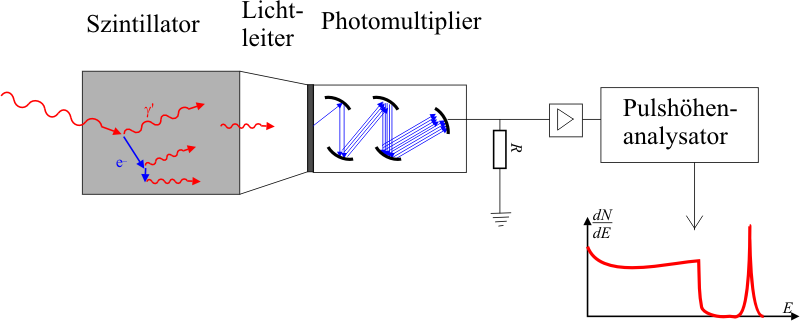
\includegraphics{Bilder/Szint.png}
 \\ Quelle: https://de.wikipedia.org/wiki/Szintillationsz\%C3\%A4hler
\newpage
\section{\underline{Auswertung}}
  \subsection{Aufgabe 1}
   Gemessene Raumbelastung: 0.2 $\mu$Sv/h \\
   Gemessene Belastung durch $^{60}{C}$ bei 0.5 m Entfernung: 0.5 $\mu$Sv/h \\
   \"Aquivalenzdosis/Jahr = Dosis/h $\cdot$ 24 $\cdot$ 365 = Dosis/h $\cdot$ 8.760 \\
   $\rightarrow$ Raumbelastung/Jahr = 1.752 mSv, $^{60}{C}$-Belastung/Jahr = 4.380 mSv \\
   Somit l\"agen wir selbst bei ein-Jahr-langer aussetzung noch unter dem Grenzwert,
   und k\"onnen daher unbesorgt experimentieren. Da die anderen strahler
   ($^{137}{Ca}$=0.3$\mu$Sv/h,$^{22}{Na}$=0.4$\mu$Sv/h, $^{241}{Am}$=0.3$\mu$Sv/h) geringer strahlen als
   $^{60}{C}$ k\"onnen wir wissen das diese auch unter dem Grenzwert liegen.
  \subsection{Aufgabe 2}
   Zur Kalibrierung des Spektrometers verwenden wir den Photopeak von $^{137}{Cs}$, von dem wir aus dem Skript wissen,
   das sein Energieniveau bei 662keV liegt. Er liegt in unserer Messung bei Kanalnummer 1922. 
    \begin{align}
     662keV \rightarrow 1922 \\
     \leftrightarrow 0.344keV \rightarrow 1
    \end{align}
   Somit wissen wir nun, das der dimensionslose Kanalnummerwert lediglich mit 0.344keV multipliziert werden muss um das zugeh\"orige Energieniveau
   herauszufinden.
  \subsection{Aufgabe 3}
   Der Vernichtungspeak von $^{22}{Na}$ liegt laut unserer Messung bei Kanal 1499. Mit 0.334keV Multipliziert ergibt dies 501keV. Laut der Einsteinschen Relation
   $E={m}_{e}c^2$ entstehen bei der Vernichtungsstrahlung zwei $\gamma$-Quanten von je 511keV. Wir liegen also mit einer Abweichung von 10keV erstaunlich genau.
  \subsection{Aufgabe 4}
   Um die Aufl\"osung des Detektors zu bestimmen, wird die Anzahl ${n}_{e}$ der Elektronen die im
   Photomultiplier von einem auftreffendem Photon ausgel\"ost werden bestimmt. ${n}_{e}$ wird \"uber die 
   Energie und die Halbwertsbreite des Photopeaks berechnet (hier von $^{137}{Cs}$):
    \begin{align}
     {n}_{e} = {\left(\frac{E}{{\Delta}E}\right)}^{2} = {\left(\frac{622}{87}\right)}^{2} \approx
     51
    \end{align}
  \subsection{Aufgabe 5}
   Die Compton-Kante liegt bei unserem graphen bei 1400, also $0.334keV * 1400 \approx 468keV$.
   Nach der Streuformel ist die Energie T:
    \begin{align}
     T=\frac{{E}_{0}}{1+\frac{{m}_{0}c^{2}}{(1-\cos\theta){E}_{0}}}
     \end{align}
  \subsection{Aufgabe 6}
   In diesem Experiment wurden die Impulse der 662keV-$\gamma$-Strahlung von $^{137}{Cs}$ gemessen
   bei unterschiedlich dicken Scheiben aus Blei (in 3 mm Schritten) und Eisen (in 5 mm Schritten).
   Wie wir aus Abb.1 entnehmen k\"onnen betr\"agt die Halbwertsdicke f\"ur Eisen $4*5mm=20mm$ und 
   f\"ur Blei $2,8*3 mm = 8,4 mm$. Dies bedeutet, dass sich die Strahlung alle 20 mm respektive alle
   8,4 mm halbiert.\\
   \begin{figure}
       \caption{y:=Anzahl Impulse, x:=Eisendicke in 5mm}
       \centering
       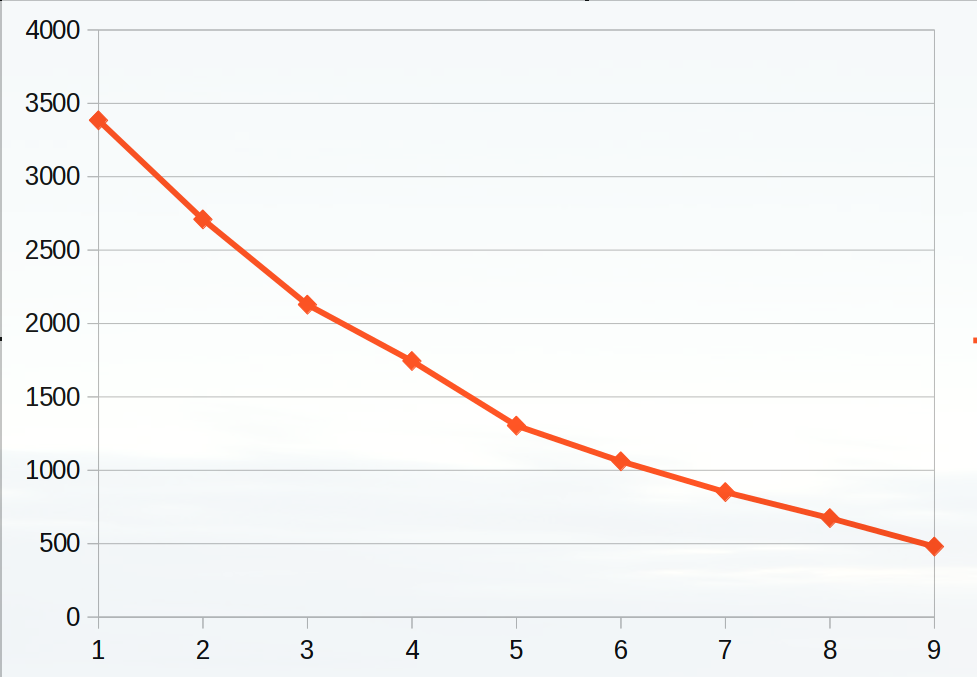
\includegraphics[scale=0.5]{Bilder/eisen.png} \\
   \end{figure}
    \begin{figure}
       \caption{y:=Anzahl Impulse, x:=Eisendicke in 3mm}
       \centering
       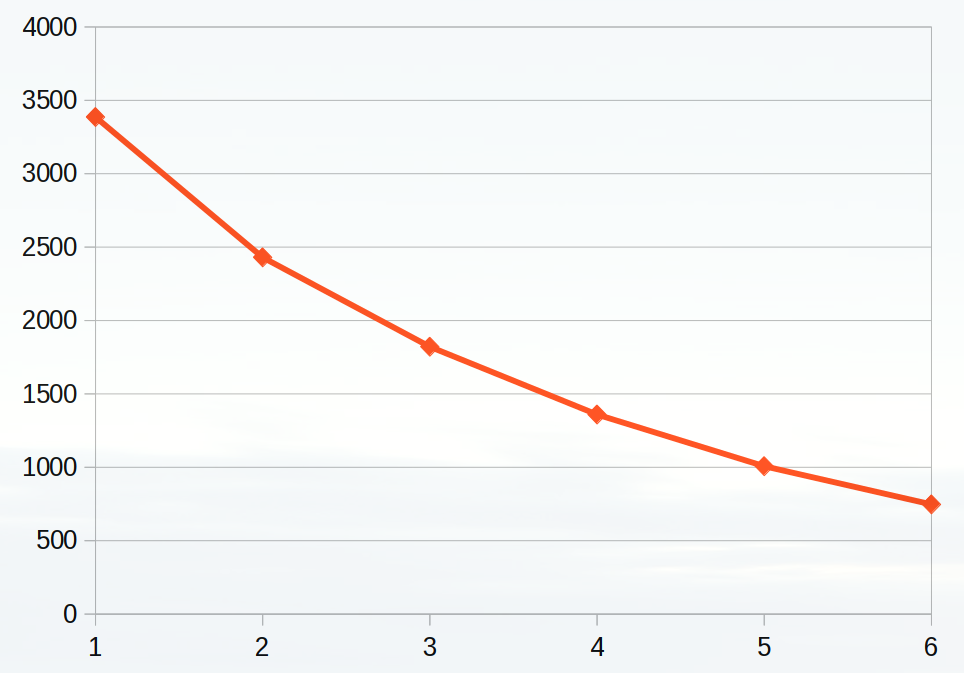
\includegraphics[scale=0.5]{Bilder/blei.png} \\
   \end{figure}





\end{document}
